\documentclass[12pt, letterpaper]{article}

\usepackage[utf8]{inputenc}
\usepackage{booktabs}
\usepackage[table,xcdraw]{xcolor}
\usepackage{hyperref}
\hypersetup{
    colorlinks=true, %set true if you want colored links
    linktoc=all,     %set to all if you want both sections and subsections linked
    linkcolor=black,  %choose some color if you want links to stand out
}
\usepackage{graphicx}
\graphicspath{{./images/}}
\usepackage{float}

\usepackage[none]{hyphenat}

\tolerance=1
\emergencystretch=\maxdimen
\hyphenpenalty=10000
\hbadness=10000

\title{Sistema Gestione ZTL}
\author{Riccardo Maria Pesce}
\date{Anno Accademico 2019-2020}

\renewcommand{\contentsname}{Contenuti}

\begin{document}

\begin{titlepage}

\maketitle

\begin{abstract}

\noindent
In questa terza iterazione verranno implementati i 
restanti casi d'uso, rifinito il software per 
tenere in considerazione gli utenti senza ID.
Vedremo di più dopo il resoconto dell'incontro con 
il cliente.
\end{abstract}
\end{titlepage}

\tableofcontents{}

\pagebreak

\section{Resoconto Iterazione 3}
Durante il meeting con il cliente, ci è stato 
fatto notare che:
\begin{itemize}
    \item Gli utenti senza dispositivo, che commettono 
    un'infrazione, non vengono sanzionati.
    \item Gli utenti che possiedono un dispositivo, possono 
    essere multati agevolmente, in quanto un'infrazione 
    verrebbe associata al codice ID del dispositivo.
\end{itemize}

\noindent
Questo ci porterà a define dei requisiti nuovi, che si andranno
ad aggiungere a quelli passati, ed integreranno/chiariranno 
quelli definiti in fase di ideazione.

\noindent 
Da un punto di vista software, le dipendenze sono ridotte 
rispetto a prima, dove il sistema centrare era responsabile 
di tutto. Tuttavia, si vedono chiaramente alcune migliorie che 
possono essere apportante, e che verranno ampiamente discusse 
nelle motivazioni progettuali.

\subsection{Richiesta Gestione Sanzioni automatica}
Come accennato nel paragrafo precedente, si vuole implementare 
nel sistema la funzionalità di sanzionare automaticamente 
gli utenti carico-scarico che commettono un infrazione.
Questa logica era prima delegata al comune, in quanto il software 
notificava (nella riga di comando), il transito irregolare.
Poi, chi di competenza multava l'utente. Adesso, dobbiamo 
implementare la logica di sanzionamento per gli utenti-carico 
scarico.

\subsection{Richiesta Riconoscimento Targhe automatico}
Per quanto concerne l'ingresso di utenti sprovvisti di 
dispositivo, il cliente richiede che il riconoscimento 
targa venga effettuato dal sistema, e non dalla revisione 
delle registrazioni, che è una gran perdita di tempo inutile.
L'implementazione dell'algoritmo verrà eseguito in parallelo 
dal dipartimento di ingegneria artificiale. Noi qui vogliamo
aggiungere la funzione di gestione accessi anche per utenti senza 
terminale, e quindi tale funzione, per adesso, sarà solamente 
simulata qui.

\section{Requisiti}

\subsection{Gestione Utenti senza Dispositivo}
Riprendendo i requisiti definiti in fase di ideazione,
andiamo ad aggiungere la nuova richiesta:
\begin{itemize}
    \item Se l'utente è residente, il sistema, 
    dopo aver acquisito il codice identificativo, 
    conferma l'ingresso ritornando quest'ultimo e 
    lascia passare il veicolo.
    \item Se l'utente è un utente Carico-Scarico, il sistema:
    \begin{enumerate}
        \item Dovrà controllare che il valico dalla 
        quale si sta entrando sia consentito al transito 
        di tale tipologia di utenti.
        \item Dovrà controllare che l'utente non 
        abbia gia usufruito dei due intervalli di 
        tempo consentiti.
    \end{enumerate}
    Solo in caso positivo, il sistema ritrasmetterà 
    il codice di identificazione come conferma del transito.
    In caso negativo, verrà ritrasmesso -1 e 
    verrà sanzionato con una sanzione di tipo 
    \emph{Transito Irregolare}.
    \item Se l'utente non ha alcun dispositivo di identificazione,
    viene registrata la sua targa e notificato il transito 
    irregolare a schermo.
\end{itemize}

\noindent
Per quanto concerne l'uscita:
\begin{itemize}
    \item Se l'utente residente, il terminale ritorna l'ID e 
    l'utente esce senza ulteriori azioni necessarie.
    \item Se l'utente è carico-scarico, il sistema controlla
    l'eventuale presenza di infrazioni all'uscita, e se 
    presenti queste verranno notificate all'utente ed 
    aggiunte al suo dispositivo (identificato da codice ID).
    \item Se l'utente non ha alcun dispositivo, verrà registrata
    la targa e notificata l'uscita al sistema centrale, 
    dove chi di dovere prenderà le giuste misure. 
\end{itemize}

\subsection{Emissione Sanzioni}
Ribadiamo che mentre per gli utenti senza targa le sanzioni 
vengono eseguite dai dipendenti (in quanto esse possono 
prevedere procedimenti al di fuori della portata del sistema),
per gli utenti carico-scarico le infrazioni vengono generate 
automaticamente dal sistema ed in seguito associate al dispositivo
che ha eseguito l'infrazione. Alla luce di ciò, definiamo:
\begin{itemize}
    \item Il sistema deve sanzionare opportunamente l'utente 
    carico-scarico colto a infrangere. 
    \item Il sistema deve accumulare per un utente le sanzioni 
    che spettano ad esso, e deve quindi provvedere l'ammontare 
    totale ed un sommario sulle irregolarità commesse.
\end{itemize}

\section{Modello dei Casi D'Uso}
A tal proposito i casi d'uso che descriveremo qui saranno
\emph{UC1} e \emph{UC2} opportunamente modificati per 
accomodare gli utenti privi di dispositivo 
(e quindi di ID), ed infine il caso d'uso 
\emph{UC5 - Sanziona Utente}.

\subsection{Caso D'Uso UC1}
\begin{itemize}
    \item \textbf{UC1:} Registra Ingresso
    \item \textbf{Portata:} Sistema Gestion ZTL
    \item \textbf{Livello:} Obiettivo utente
    \item \textbf{Pre-condizioni:} l'utente sta varcando 
    il valico d'ingresso
    \item \textbf{Garanzie di successo (Post-condizioni):} 
    l'utente (identificato) entra nella zona a traffico 
    limitato
    
    \item \textbf{Scenario principale di successo}
    \begin{itemize}
        \item L'utente, avvicinatosi al varco, 
        innesta il sistema attraverso l'invio, 
        da parte del telepass, di un codice 
        identificativo
        \item Se l'utente è residente, 
        il telepass lo lascia passare senza 
        ulteriori azioni
        \item Se l'utente non è residente, 
        il terminale è abilitato all'ingresso 
        di utenti carico-scarico e l'utente non 
        ha gia usufruito dei suoi due intervalli 
        consentiti, il sistema registra l'orario 
        d'ingresso e ritorna alla vettura il codice 
        identificativo come conferma, e lo lascia 
        passare
    \end{itemize}
    
    \item \textbf{Scenari alternativi}
    \begin{itemize}
        \item \textbf{Il varco non è 
        abilitato all'accesso degli utenti 
        carico-scarico}
        \begin{enumerate}
            \item Viene registrata l'infrazione
            \emph{Ingresso irregolare} all'utente (attraverso
            il suo ID).
        \end{enumerate}
        \item \textbf{Il transito sta avvenendo 
        in un intervallo non consentito}
        \begin{enumerate}
            \item Viene registrata l'infrazione 
            \emph{Transito Irregolare} all'utente 
            attraverso il suo ID.
        \end{enumerate}
        \item \textbf{L'utente non possiede 
        alcun dispositivo telepass}
        \begin{enumerate}
            \item Attraverso un'apposita telecamera 
            viene registrata la targa dell'utente. 
            \item Viene notificata l'infrazione 
            \emph{Transito non consentito} 
        \end{enumerate}
    \end{itemize}
    
    \item \textbf{Requisiti speciali:} Bassa latenza
    \item \textbf{Frequenza:} Ogni qualvolta un utente si 
    presenta al varco
\end{itemize}

\subsection{Caso D'Uso UC2}
\begin{itemize}
    \item \textbf{UC2:} Registra Uscita
    \item \textbf{Portata:} Sistema Gestion ZTL
    \item \textbf{Livello:} Obiettivo utente
    \item \textbf{Pre-condizioni:} l'utente si trova 
    all'interno della zona a traffico limitato
    \item \textbf{Garanzie di successo (Post-condizioni):} 
    l'utente esce dalla zona a traffico limitato
    \item \textbf{Scenario principale di successo}
    \begin{itemize}
        \item L'utente, avvicinatosi al varco d'uscita, 
        attiva il sistema attraverso l'invio, 
        da parte del telepass, di un codice identificativo
        \item Se l'utente è residente, il telepass lo 
        lascia uscire senza ulteriori azioni.
        \item Se l'utente è carico-scarico, il varco di uscita 
        è quello abilitato a tali utenti e non ha sostato per 
        più di un'ora, il sistema registra lo rimuove 
        semplicemnte da una determinata lista di utenti 
        carico-scarico all'interno della ZTL e ritorna alla 
        vettura il codice identificativo come conferma, e 
        lo lascia passare
        \item Se l'utente è sprovvisto di dispositivo,
        viene lasciato passare, in quanto comunque il 
        suo transito è stato registrato. Viene solamente
        notificata l'uscita.
    \end{itemize}    
    \item \textbf{Scenari alternativi}
    \begin{itemize}
        \item \textbf{L'utente è rimasto per più del 
        tempo consentito}
        \begin{enumerate}
            \item Viene registrata una multa di tipo 
            \emph{Transito in Eccesso} all'utente (attraverso
            il suo ID).
        \end{enumerate}
    \end{itemize}
    
    \item \textbf{Requisiti speciali:} Bassa latenza
    \item \textbf{Frequenza:} Ogni qualvolta un utente 
    si presenta al varco d'uscita 
\end{itemize}

\subsection{Caso D'Uso UC5}
\begin{itemize}
    \item \textbf{UC5:} Sanziona Utente
    \item \textbf{Portata:} Sistema Gestion ZTL
    \item \textbf{Livello:} Obiettivo utente
    \item \textbf{Pre-condizioni:} l'utente ha commesso 
    un'irregolarità.
    \item \textbf{Garanzie di successo (Post-condizioni):} 
    l'utente viene sanzionato, associando al suo dispositivo
    una sanzione.
     
    \item \textbf{Scenario principale di successo}
    \begin{itemize}
        \item Se l'utente sta eseguendo l'ingresso:
        \begin{itemize}
            \item Se l'ingresso è fuori intervallo,
            il sistema eroga una sanzione "Transito 
            Irregolare"
            \item Se l'ingresso è gia avvenuto,
            e l'utente quindi sta eseguendo di 
            nuovo l'accesso, il sistema eroga una 
            sanzione "Transito Extra".
            \item Se l'ingresso avviene da terminale 
            residente, viene erogata una multa di tipo 
            "Accesso irregolare".
        \end{itemize} 
        \item Se l'utente sta eseguendo l'uscita:
        \begin{enumerate}
            \item Se l'uscita avviene dopo lo 
            scattare dell'ora, il sistema registra 
            la sanzione con l'ammontare determinato 
            secondo la relativa regola di business 
            definita sotto. Verra erogata una multa 
            di tipo "Transito Extra".
        \end{enumerate} 
    \end{itemize}
    
    \item \textbf{Scenari alternativi}
    \begin{itemize}
        \item \textbf{L'utente non ha dispositivo ID}
        \begin{itemize}
            \item Viene registrata la targa attraverso
            la telecamera e viene notificato il 
            transito, sia esso in ingresso o uscita,
            al sistema centrale da terminale.
        \end{itemize}
    \end{itemize}
    
    \item \textbf{Requisiti speciali:} Bassa latenza
    \item \textbf{Frequenza:} Sempre potenzialmente
    (ogni volta che viene commessa un'infrazione).
\end{itemize}

\section{Regole di Business}
Si rende necessario, alla luce dei requisiti e dei casi 
d'uso formulati, aggiungere ulteriori regole di business,
specie per quanto riguarda il computo delle sanzioni.
Definiamo quindi:
\begin{enumerate}
    \item \textbf{Regola R6:} Il sistema sanziona esegue sanzioni
    relative al transito nella zona a traffico limitato.
    \item \textbf{Regola R7:} L'entrata al di fuori dell'intervallo 
    concesso agli utenti carico-scarico verrà multana con 
    una sanzione "TRANSITO IRREGOLARE" dal valore di 50 euro.
    \item \textbf{Regola R8:} L'entrata extra oltre a quella 
    concessa giornalmente viene multata con una sanzione 
    "TRANSITO EXTRA" dal valore di 30 euro.
    \item \textbf{Regola R9:} L'uscita al di fuori dell'ora 
    concessa ammonta a 15 euro e viene descritta come 
    "TRANSITO ECCESSIVO".
    \item \textbf{Regola R10:} Le multe che concernono gli utenti 
    senza targa sono a carico degli impiegati comunali in quanto 
    la sanzione, essendo grave, può portare a conseguenze fuori 
    dalla portata dell'applicazione.
    \item \textbf{Regola R11:} L'infrazione che commete l'utente 
    carico-scarico che entra, anche nel regolare intervallo,
    da un terminale per i soli residenti viene indicata con 
    "ACCESSO IRREGOLARE" e viene multata con 10 euro.
\end{enumerate}

\section{Modello di Dominio}
Il modello di dominio per questa iterazione si può definire 
in termini di quello dell'iterazione precedente, con l'aggiunta 
della classe concettuale \emph{Sanzione}, ed il rifinimento 
di alcune associazioni: per esempio, \emph{Terminale} autentica 
\emph{Autenticatore} attraverso la creazione di un'istanza di 
\emph{Accesso} e sanziona essa attraverso la creazione di un'istanza
\emph{Sanzione}. Queste associazioni vengono rappresentate 
attraverso una linea che punta alla linea che connette le due 
classi da associare.
\begin{figure}[H]
    \centering
    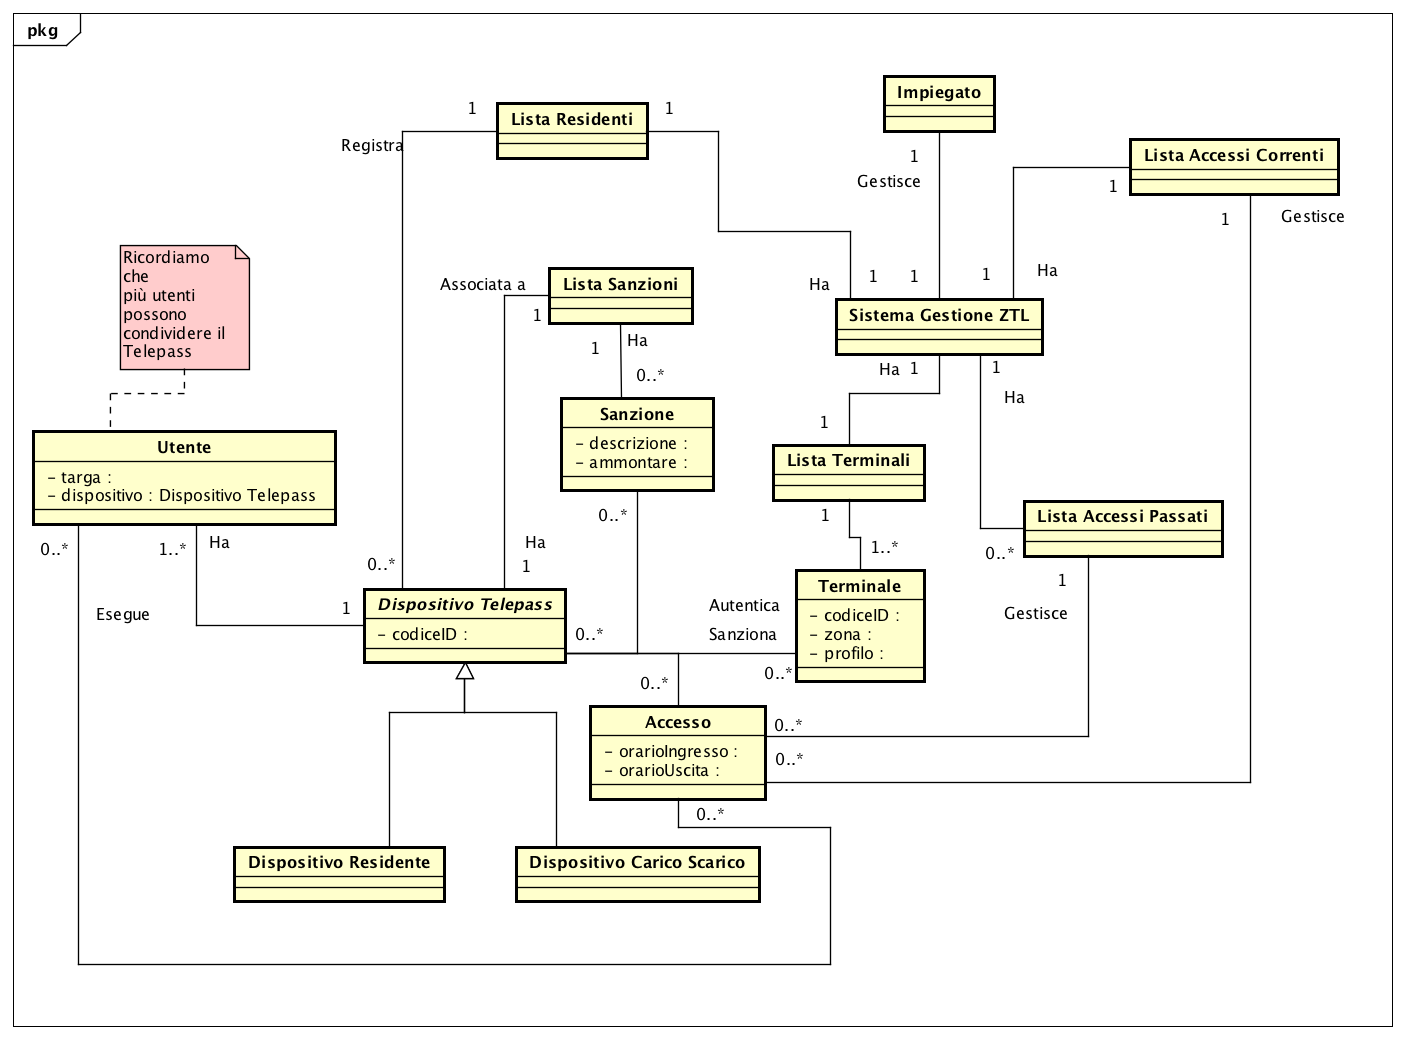
\includegraphics[scale=0.35]{ModelloDominio}
\end{figure}

\noindent
Per un maggior dettaglio grafico, consultare i file allegati
\texttt{/diagrams/ModelloDominio.asta} oppure
\texttt{/images/ModelloDominio.png}.
La lista delle sanzioni è unica per ogni utente, anche se 
come per gli altri moduli gestori, in fase di progetto 
sicuramente seguiremo la stessa architettura e quindi 
utilizzeremo un gestore per le sanzioni.

\section{Diagrammi di Sequenza di Sistema}
Riportiamo i diagrammi di sequenza di sistema 
dei casi d'uso \emph{UC1},
\emph{UC2} ed \emph{UC5 
- Emetti Sanzione}. Gli altri diagrammi 
sono pressochè invariati (solo le classi sono 
variate).

\subsection{UC1}
Introduciamo il caso in cui l'utente è senza 
dispositivo.
\begin{figure}[H]
    \centering
    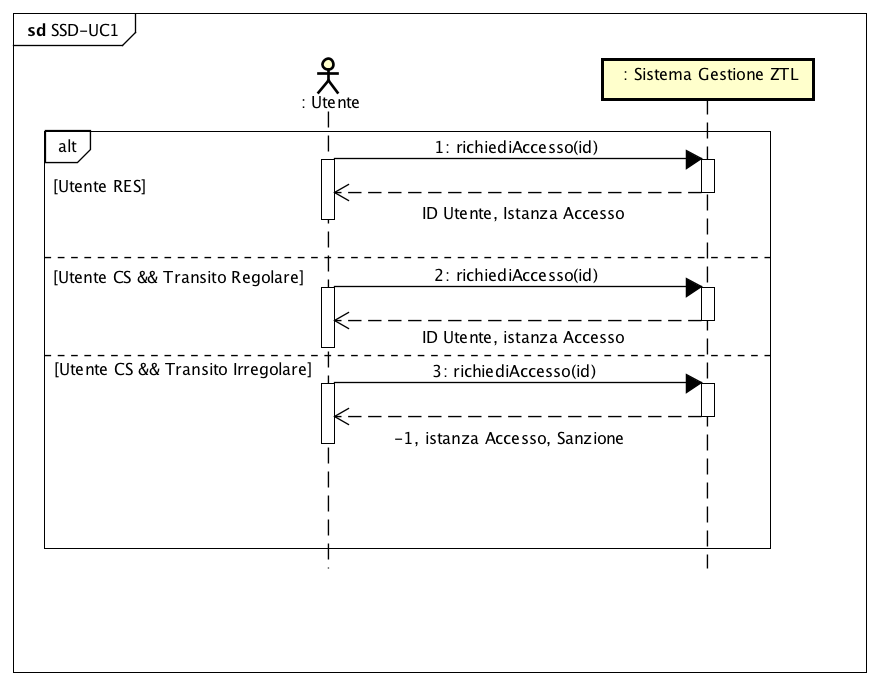
\includegraphics[scale=0.50]{UC1-SSD}
\end{figure}

\noindent
Introduciamo il caso in cui l'utente è senza 
dispositivo.
\begin{figure}[H]
    \centering
    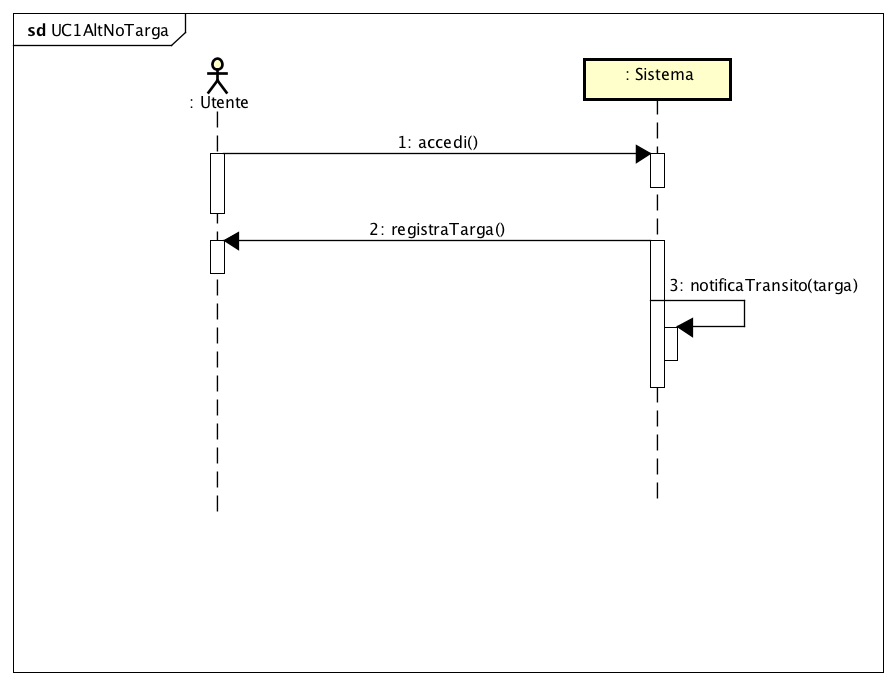
\includegraphics[scale=0.50]{UC1NoTarga}
\end{figure}

\noindent
Da notare come si è voluto enfatizzare che 
la notifica del transito viene eseguita 
internamente al sistema.

\subsection{UC2}
\begin{figure}[H]
    \centering
    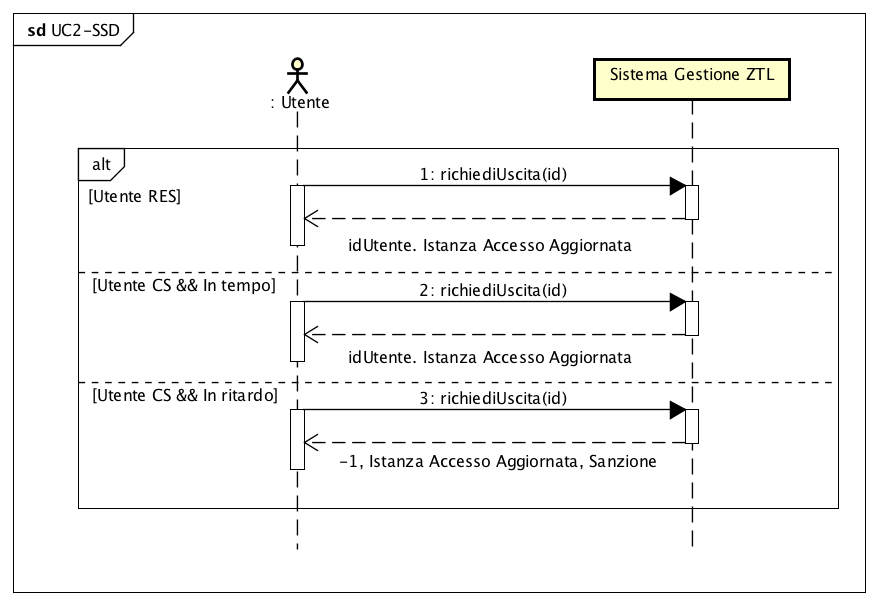
\includegraphics[scale=0.50]{UC2-SSD}
\end{figure}

\noindent 
Introduciamo anche qui il caso in cui 
l'utente è senza dispositivo.
\begin{figure}[H]
    \centering
    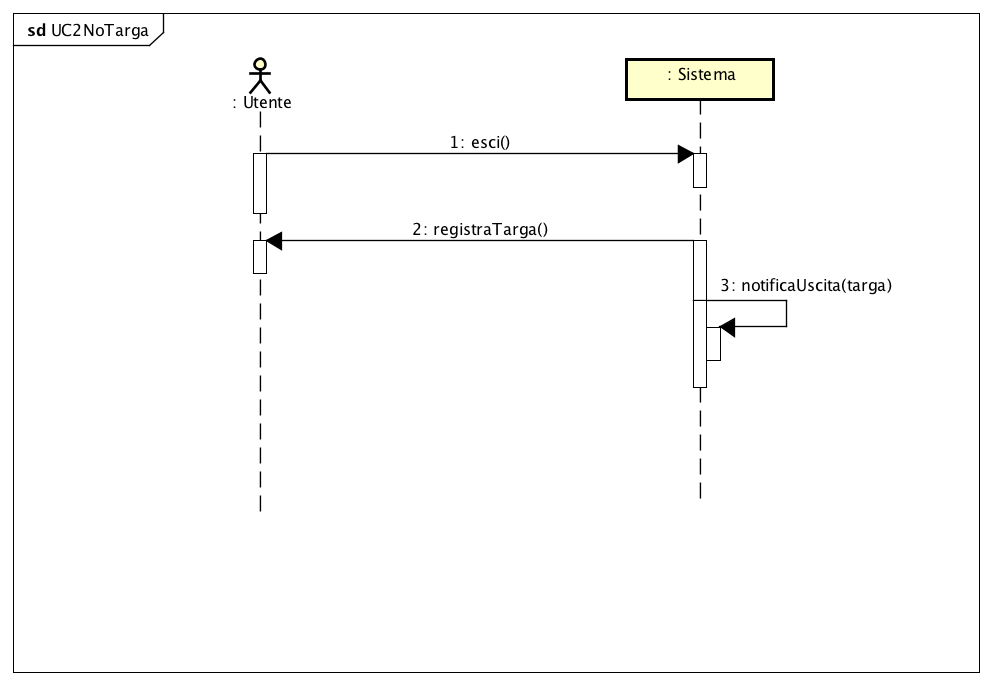
\includegraphics[scale=0.50]{UC2NoTarga}
\end{figure}

\noindent
Anche qui enfatizziamo come la notifica 
d'uscita sia eseguita internamente.

\subsection{UC5 - Emetti Sanzione}
Tale caso d'uso, a livello di interazioni,
è collegato ai casi d'uso \emph{UC1} ed 
\emph{UC2}. Temporalmente esso avviene 
dopo la creazione dell'istanza d'ingresso/
aggiornamento della stessa in uscita.
Lo rappresenteremo dunque come un caso a 
se stante, riassumento i casi d'uso \emph{UC1}
ed \emph{UC2} con i messaggi \texttt{entra()} ed 
\texttt{esci()} rispettivamente.

\noindent
Nel caso che l'utente stia commettendo un 
infrazione in ingresso, avremo il seguente
diagramma:
\begin{figure}[H]
    \centering
    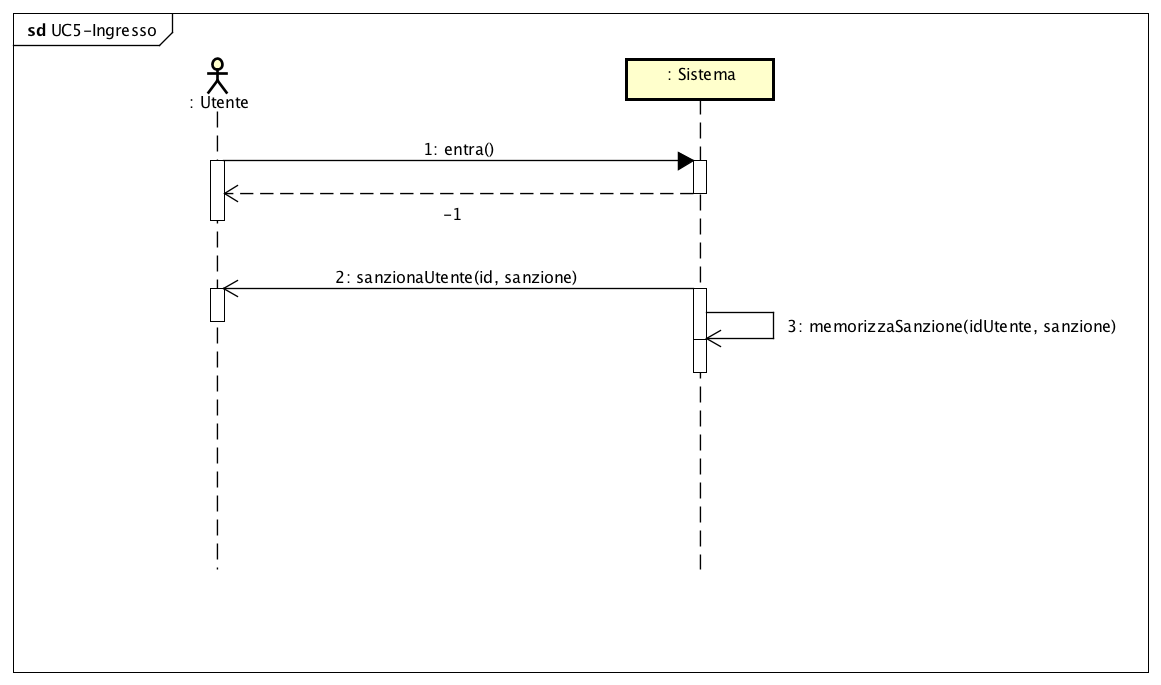
\includegraphics[scale=0.40]{UC5-Ingresso}
\end{figure} 

\noindent
Mentre nel caso d'uscita avremo:
\begin{figure}[H]
    \centering
    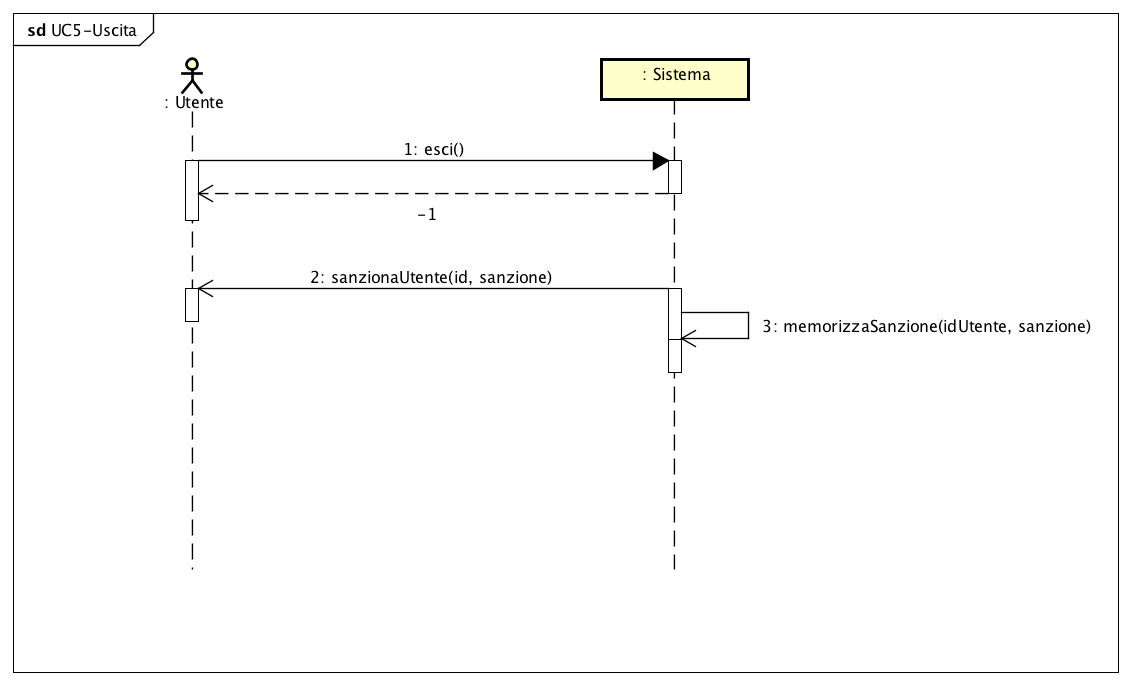
\includegraphics[scale=0.40]{UC5-Uscita}
\end{figure} 

\noindent
L'emissione della sanzione consta di due 
azioni fondamentali: la notifica all'utente
e la registrazione in una lista interna al 
sistema, in modo tale che si possa tenere 
traccia. Dettagli sull'implementazione vanno 
lasciati alla fase di progettazione, in questa 
fase vogliamo solo indicare quel che l'operazione 
fa, e nel prossimo paragrafo definiremo le 
operazioni più dettagliatamente.

\section{Contratti delle Operazioni}

\subsection{CO5 - \texttt{notificaIngressoTarga()}}
\begin{itemize}
    \item \textbf{Operazione:} 
    \texttt{notificaIngressoTarga(String : targa)}
    \item \textbf{Riferimenti:} Caso d'uso UC1
    \item \textbf{Pre-condizioni:} un utente senza 
    dispositivo si trova in procinto di accedere 
    nella zona a traffico limitato
    \item \textbf{Post-condizioni:} l'utente 
    è entrato nella zona a traffico limitato, 
    ed il suo transito irregolare è stato 
    notificato
\end{itemize}

\subsection{CO6 - \texttt{notificaUscitaTarga()}}
\begin{itemize}
    \item \textbf{Operazione:} 
    \texttt{notificaUscitaTarga(String : targa)}
    \item \textbf{Riferimenti:} Caso d'uso UC2
    \item \textbf{Pre-condizioni:} un utente senza 
    dispositivo si trova in procinto di uscire 
    dalla zona a traffico limitato
    \item \textbf{Post-condizioni:} l'utente 
    è uscito e l'uscita è stata notificata
\end{itemize}

\subsection{CO7 - \texttt{emettiSanzione()}}
\begin{itemize}
    \item \textbf{Operazione:} 
    \texttt{emettiSanzione(int : idUtente, Sanzione : sanzione)}
    \item \textbf{Riferimenti:} Caso d'uso UC5
    \item \textbf{Pre-condizioni:} l'utente ha commesso 
    un'infrazione in ingresso/uscita nella zona a traffico 
    limitato
    \item \textbf{Post-condizioni:} l'utente 
    è entrato/uscito, e la relativa sanzione è stato 
    notificata e registrata
\end{itemize}

\section{Diagrammi di Interazione}

\subsection{UC1 - Registra Ingresso}
Se l'ingresso avviene regolarmente con dispositivo,
vale il seguente diagramma di interazione.
Vale sempre la regolare secondo il quale la variabile 
\texttt{codiceRitorno} sia pari al codice ID dell'utente 
se l'accesso sta avvenendo in piena regolarità, -1 
altrimenti. I controlli della regolarità del transito 
vengono fatti dal gestore degli accessi.
Osserviamo come i gestori funzionano da intermediari, 
in quanto inoltrano le richieste dei singoli componenti 
verso il sistema centrale.
Inoltre, si vuole notare l'applicazione del pattern 
\emph{Command}. Si vuole delegare il ruolo 
dell'\emph{Invoker} al terminale, ed il ruolo del 
\emph{Receiver} al gestore dei terminali, che, 
come gia detto, inoltrerà la richiesta al sistema 
centrale che medierà la stessa all'opportuno gestore.
Viene passata l'istanza di richiesta stessa che il 
gestore degli accessi userà per inizializzare 
l'istanza d'accesso stesso.
\begin{figure}[H]
    \centering
    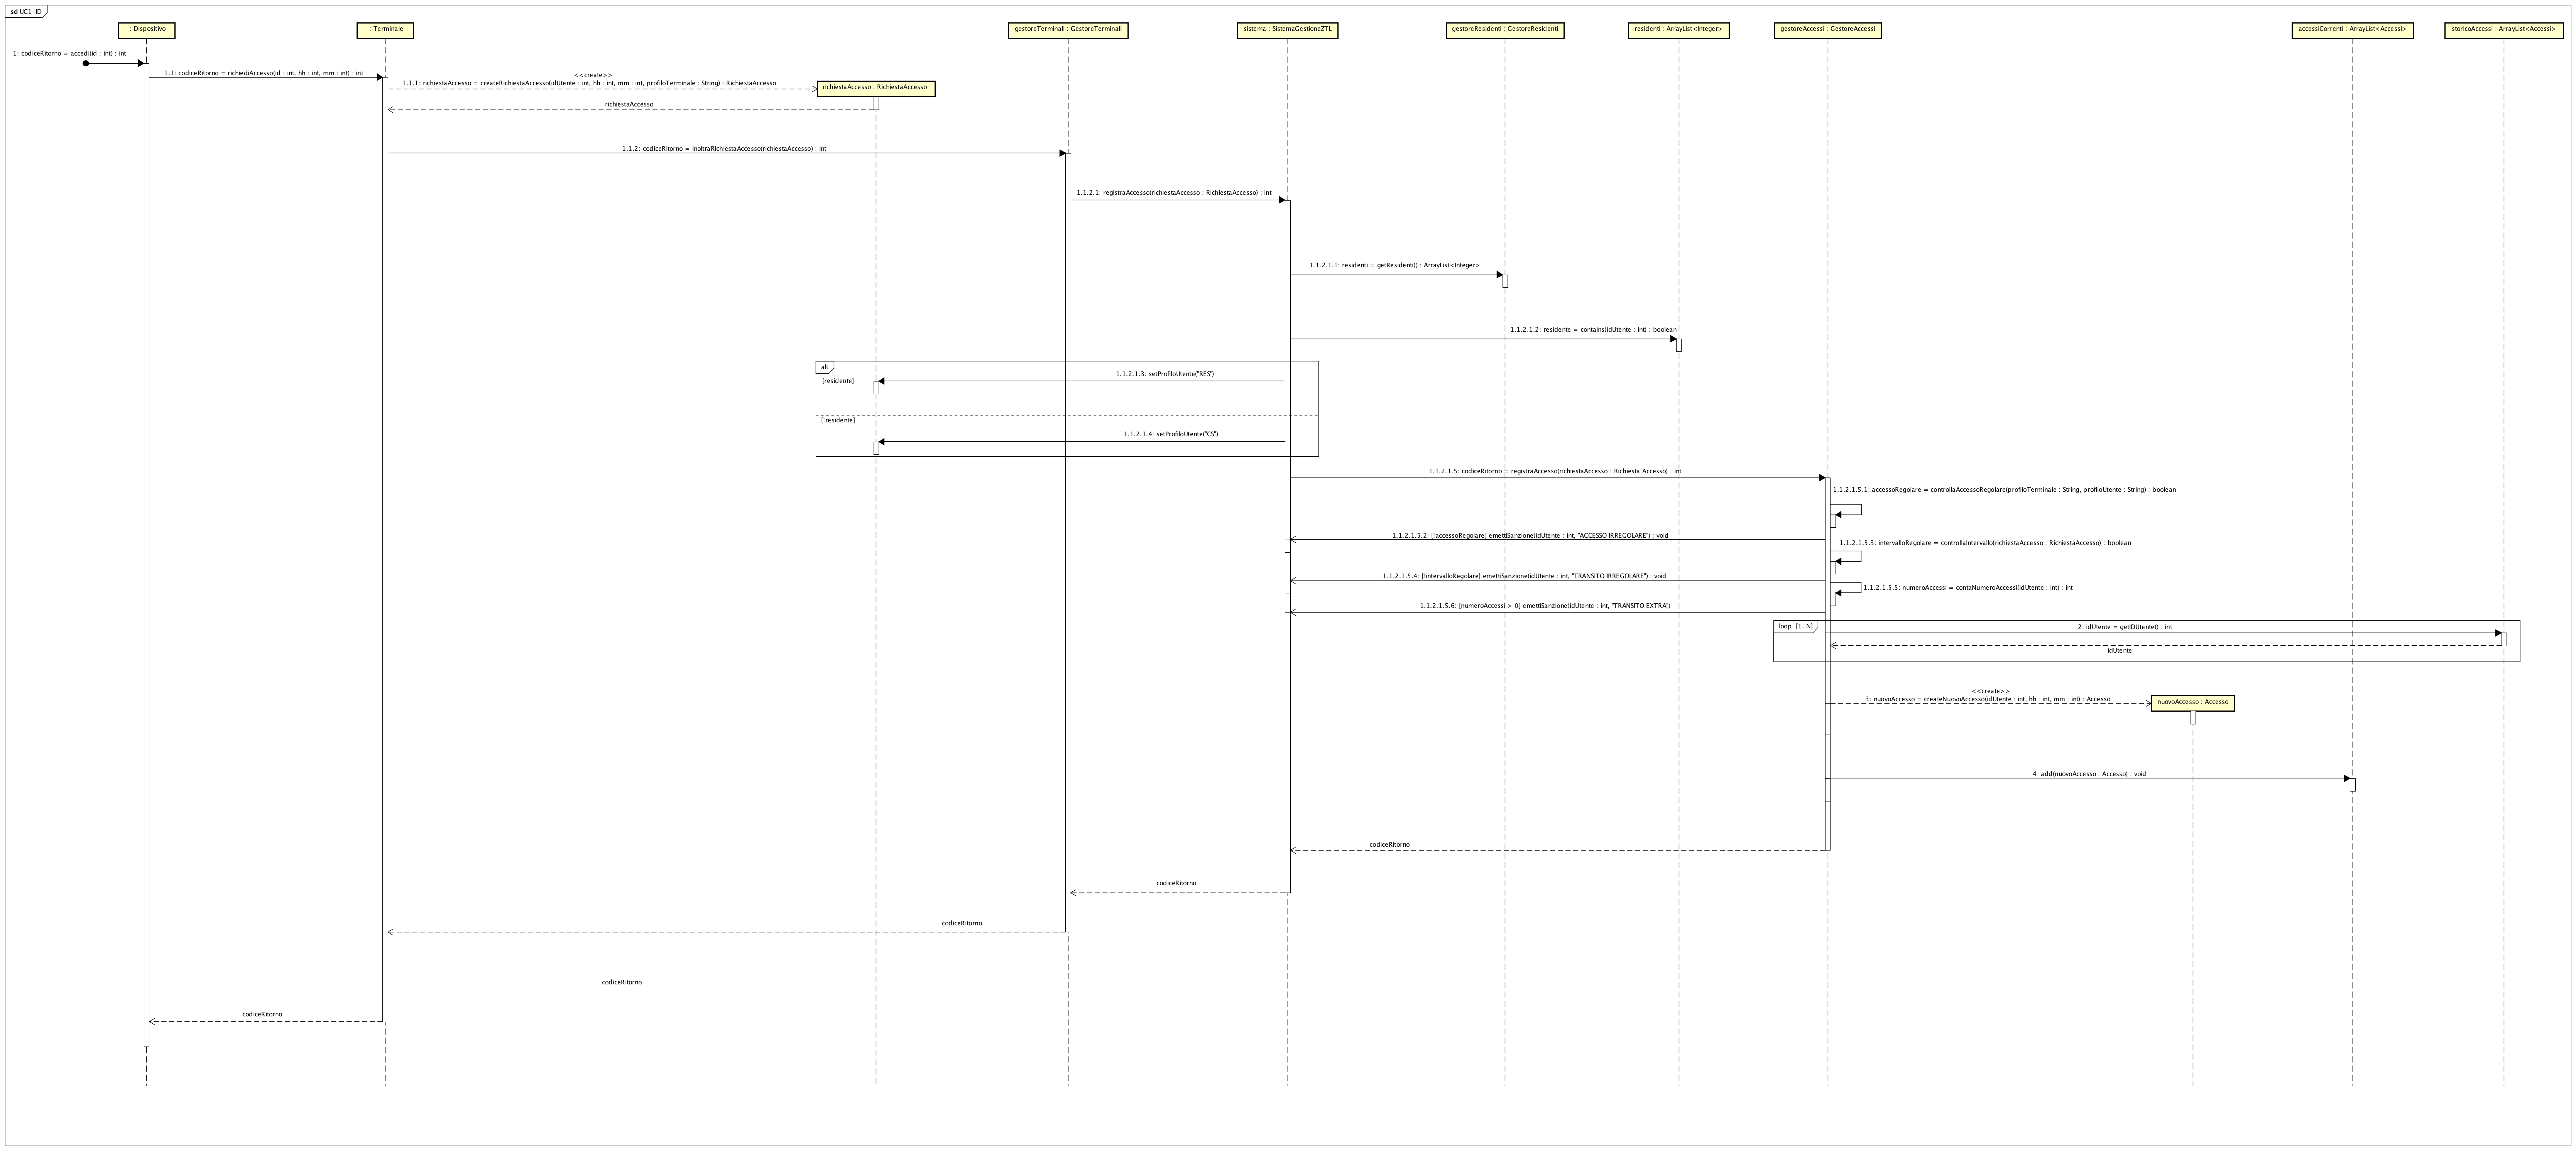
\includegraphics[scale=0.07]{UC1-ID}
\end{figure} 

\noindent
Per un maggior dettaglio grafico, fare riferimento alla figura 
\texttt{UC1-ID.png} od il file \texttt{UC1-ID.asta}.

\noindent
E' di grande importanza mostrare le interazioni che avvengono 
all'ingresso dell'utente sprovvisto di dispositivo.
\begin{figure}[H]
    \centering
    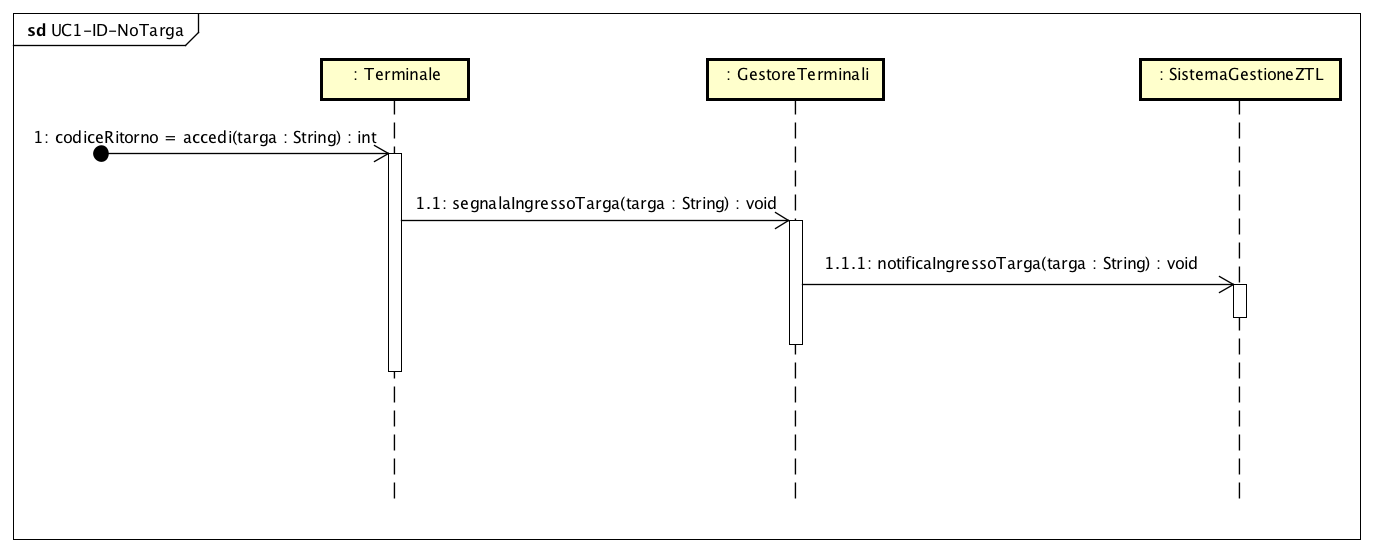
\includegraphics[scale=0.40]{UC1-ID-NoTarga}
\end{figure} 

\noindent
A differenza del caso precedente, qui il terminale segnala
l'ingresso irregolare dell'utente senza dispositivo. 
Le conseguenze sono fuori dalla portata dell'applicazione, 
pertanto il nostro ruolo si limita a segnalare l'ingresso e
l'uscita.

\subsection{UC2 - Registra Uscita}
\begin{figure}[H]
    \centering
    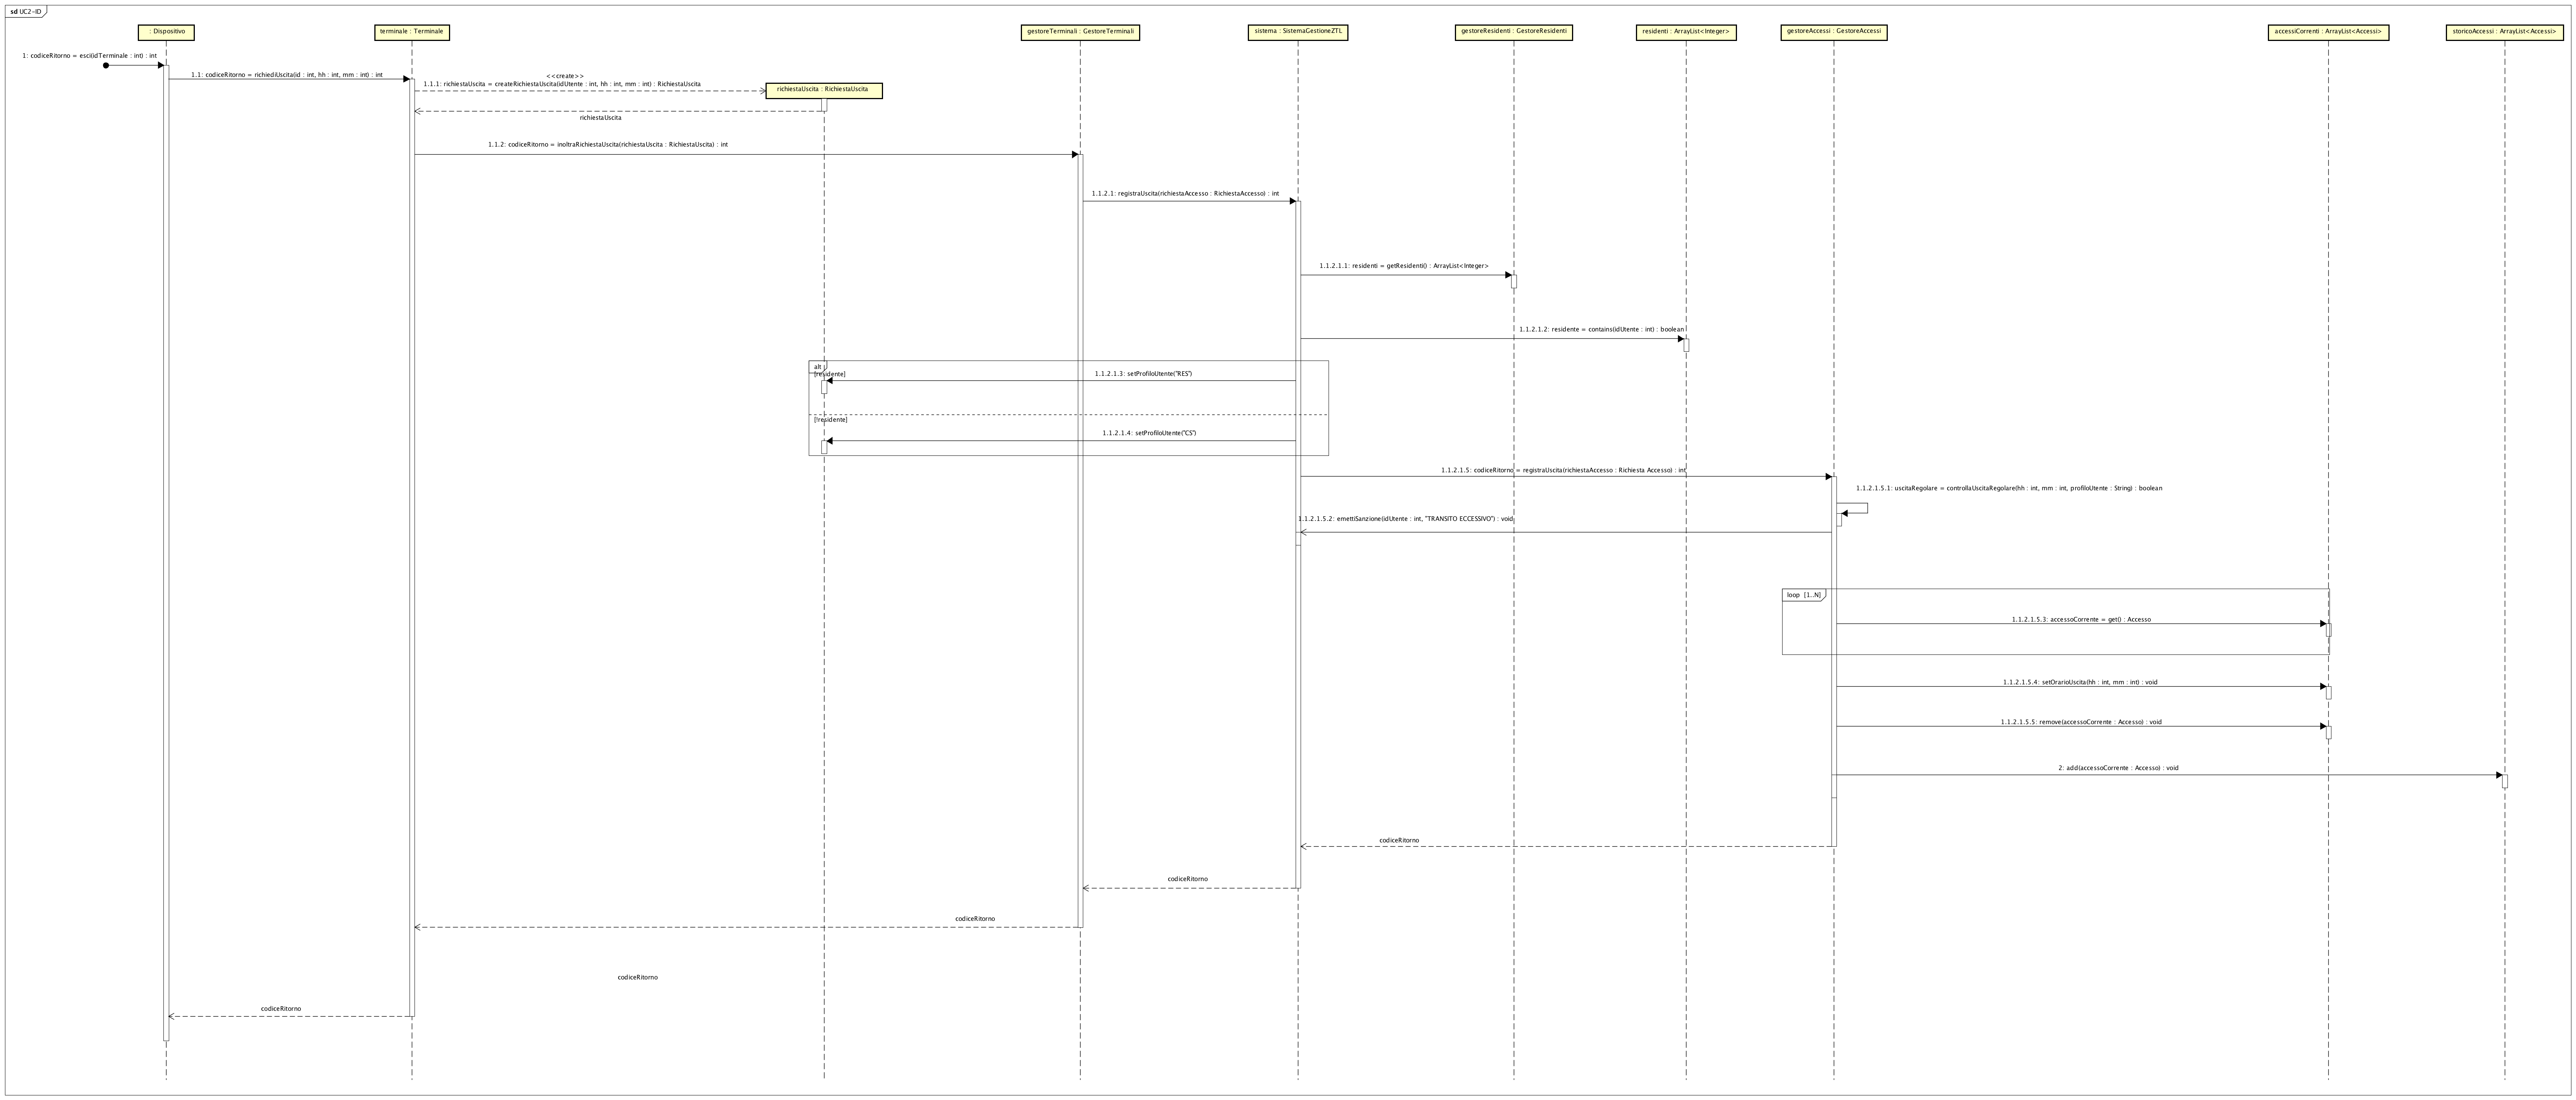
\includegraphics[scale=0.07]{UC2-ID}
\end{figure}

\noindent
Per un maggior dettaglio grafico, fare riferimento alla figura 
\texttt{UC2-ID.png} od il file \texttt{UC2-ID.asta}.

\noindent
Similmente al caso d'uso precedente, mostriamo il 
diagramma d'interazione per lo scenario in cui 
l'utente è senza dispositivo.

\begin{figure}[H]
    \centering
    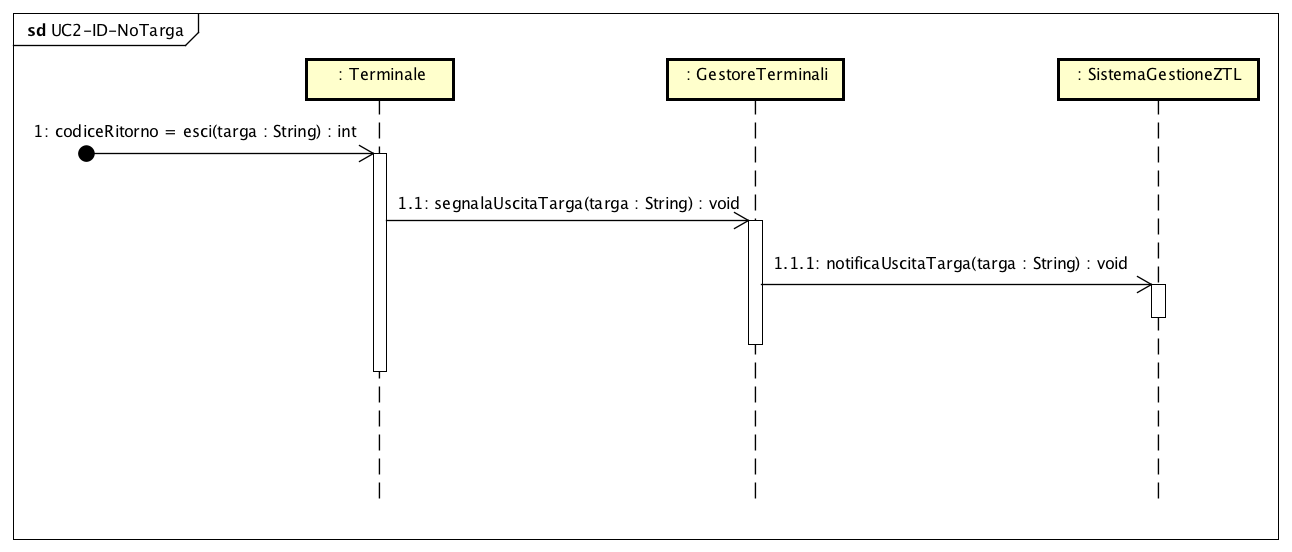
\includegraphics[scale=0.40]{UC2-ID-NoTarga}
\end{figure} 

\noindent
Si noti come, analogamente al caso precedente,
in caso di infrazione, il gestore degli accessi 
chiama il sistema centrale.
Il seguito a tale chiamata è illustrato nell'opportuno 
diagramma di interazione per il caso d'uso \emph{UC5}.

\subsection{UC3 - Gestisci Terminali}
Il caso d'uso \emph{UC3.1} presenta il seguente diagramma
d'interazione
\begin{figure}[H]
    \centering
    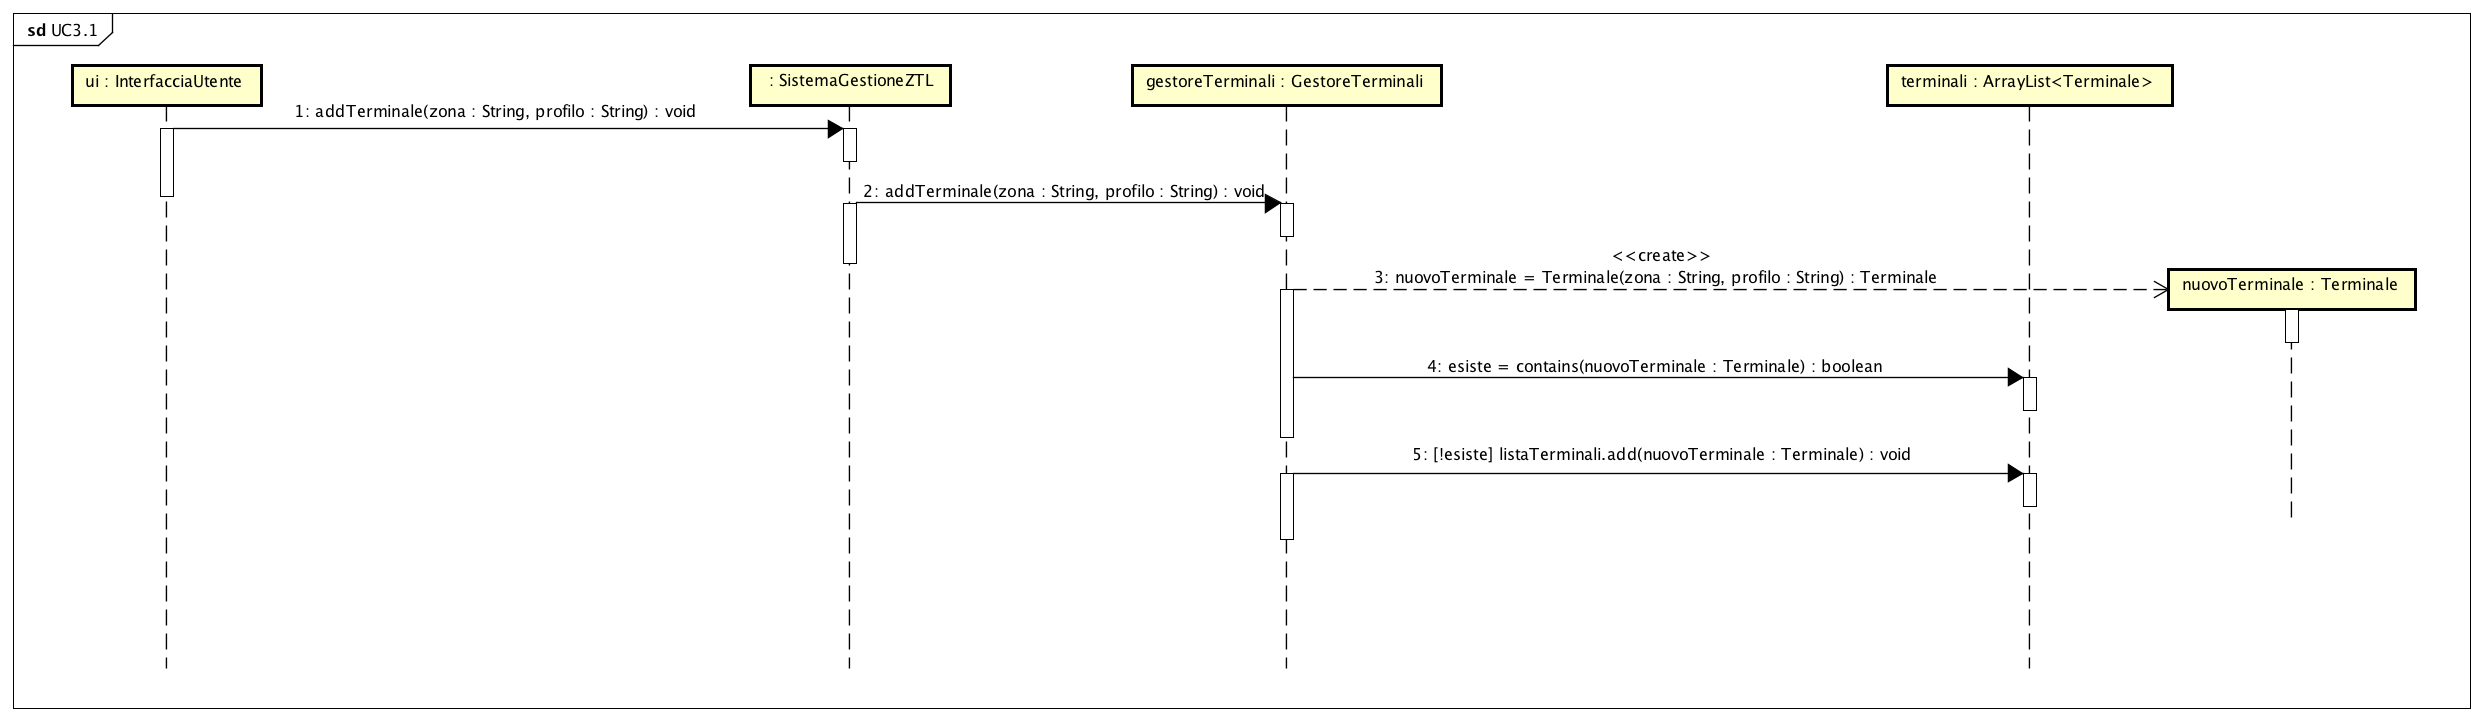
\includegraphics[scale=0.18]{UC3.1-ID}
\end{figure} 

\noindent
Se il terminale esiste gia, verrà stampato a schermo un 
messaggio.

\noindent
Passiamo al caso d'uso \emph{UC3.2}, quando utilizziamo
la rimozione per codice id:

\begin{figure}[H]
    \centering
    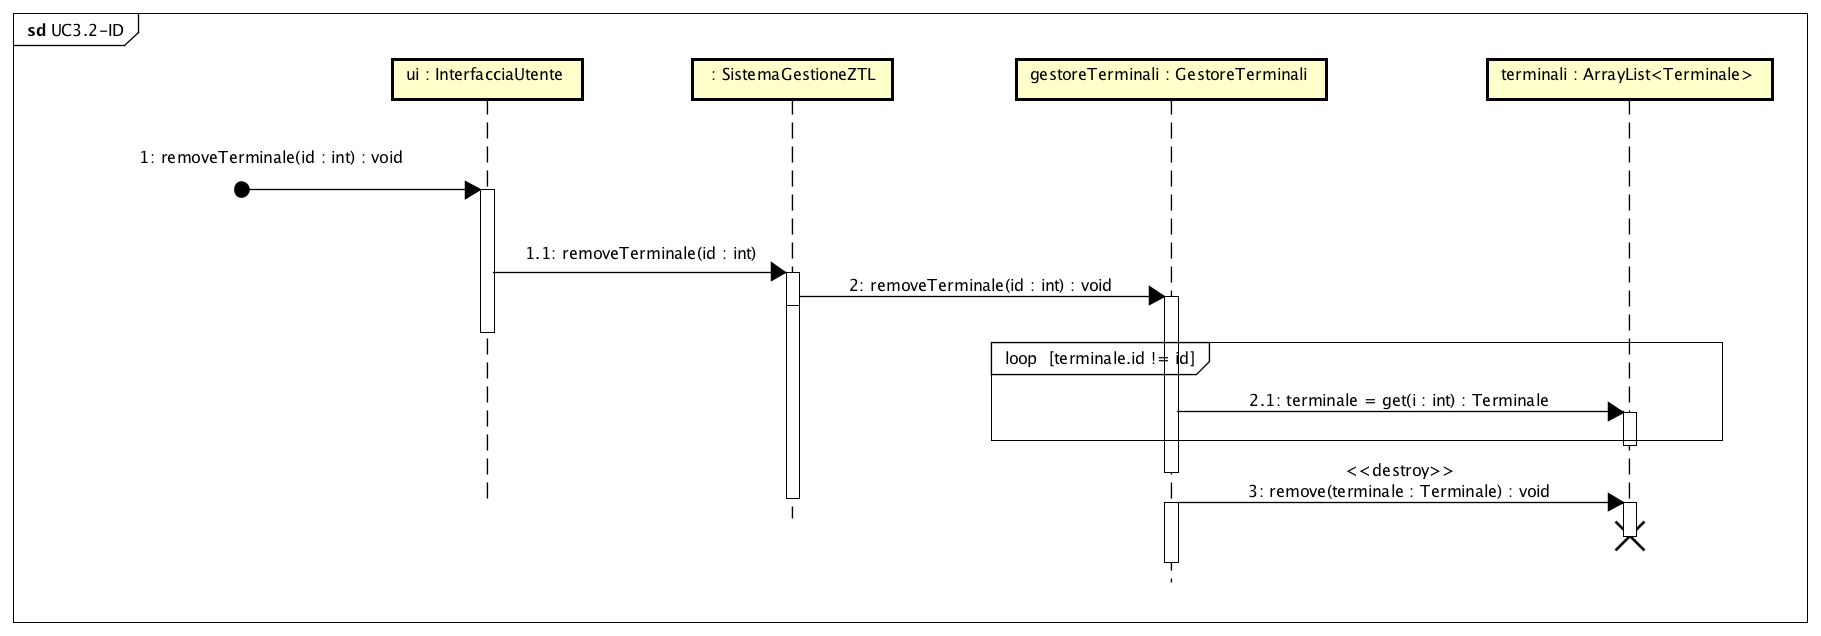
\includegraphics[scale=0.25]{UC3.2-ID-ID}
\end{figure} 

\noindent
Quando eseguiamo la rimozione per zona, si avrà il seguente:

\begin{figure}[H]
    \centering
    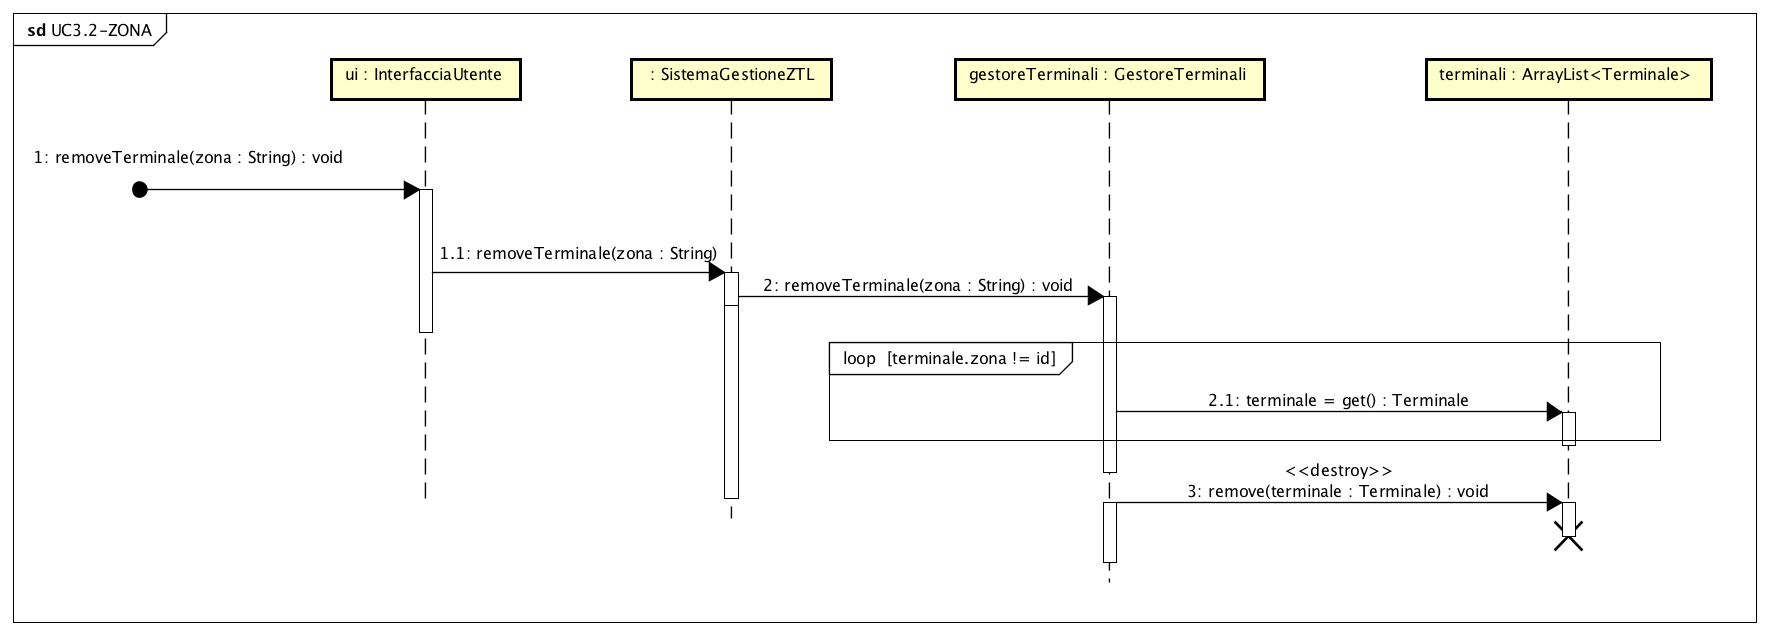
\includegraphics[scale=0.25]{UC3.2-ZONA-ID}
\end{figure} 

\subsection{UC4 - Gestisci Residenti}
Per il caso d'uso \emph{UC4.1} abbiamo il seguente 
diagramma di sequenza:
\begin{figure}[H]
    \centering
    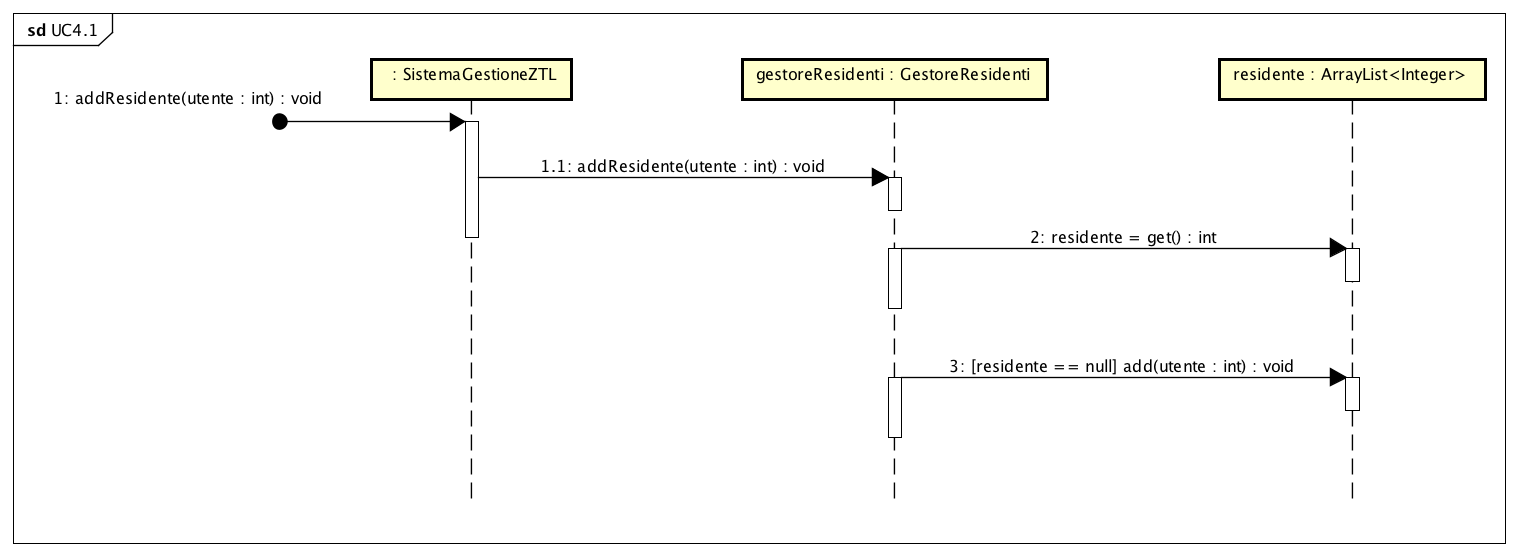
\includegraphics[scale=0.30]{UC4.1-ID}
\end{figure} 

\noindent
Mentre per il caso d'uso \emph{UC4.2} abbiamo:
\begin{figure}[H]
    \centering
    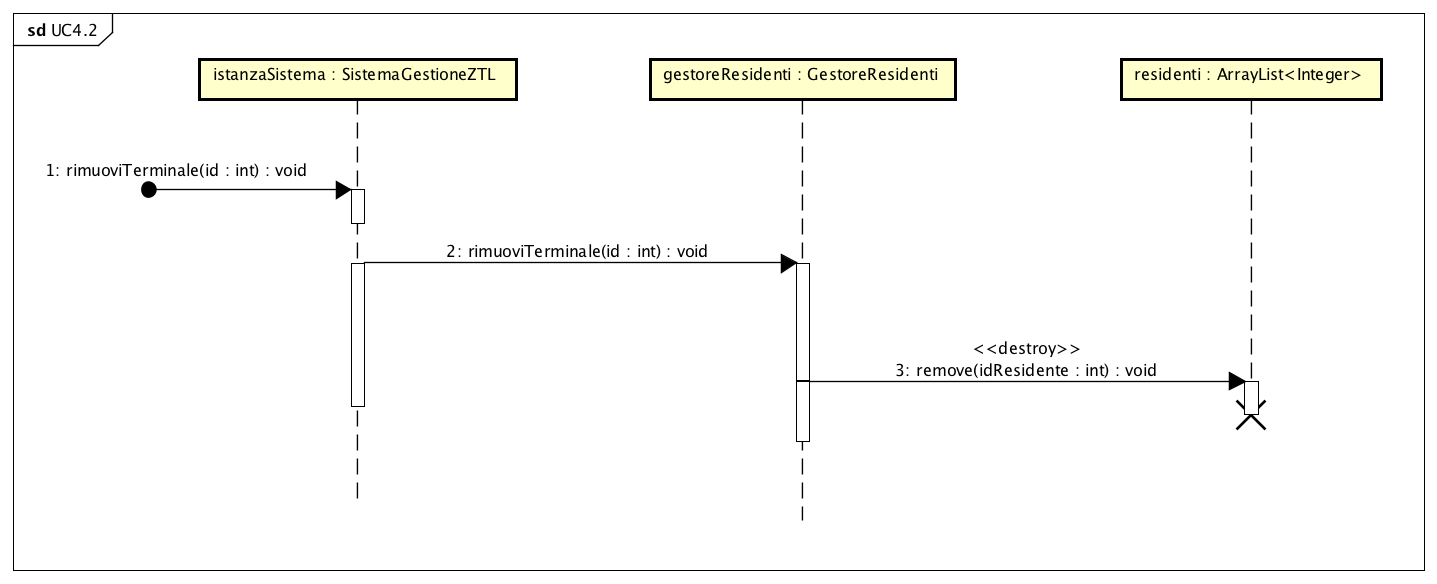
\includegraphics[scale=0.30]{UC4.2-ID}
\end{figure} 

\subsection{UC5 - Emetti Sanzione}
\begin{figure}[H]
    \centering
    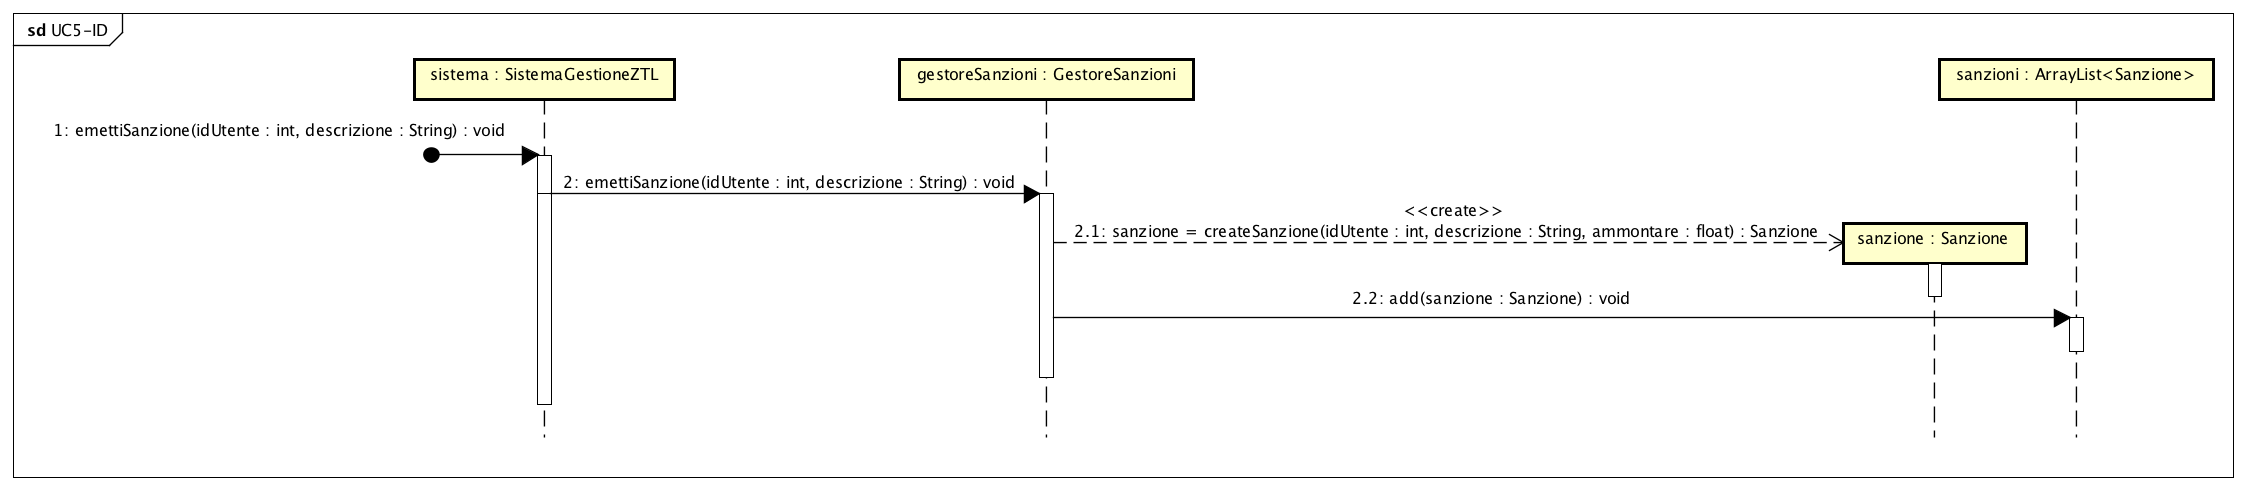
\includegraphics[scale=0.20]{UC5-ID}
\end{figure} 

\section{Diagrammi delle Classi Progettuali}
\begin{figure}[H]
    \centering
    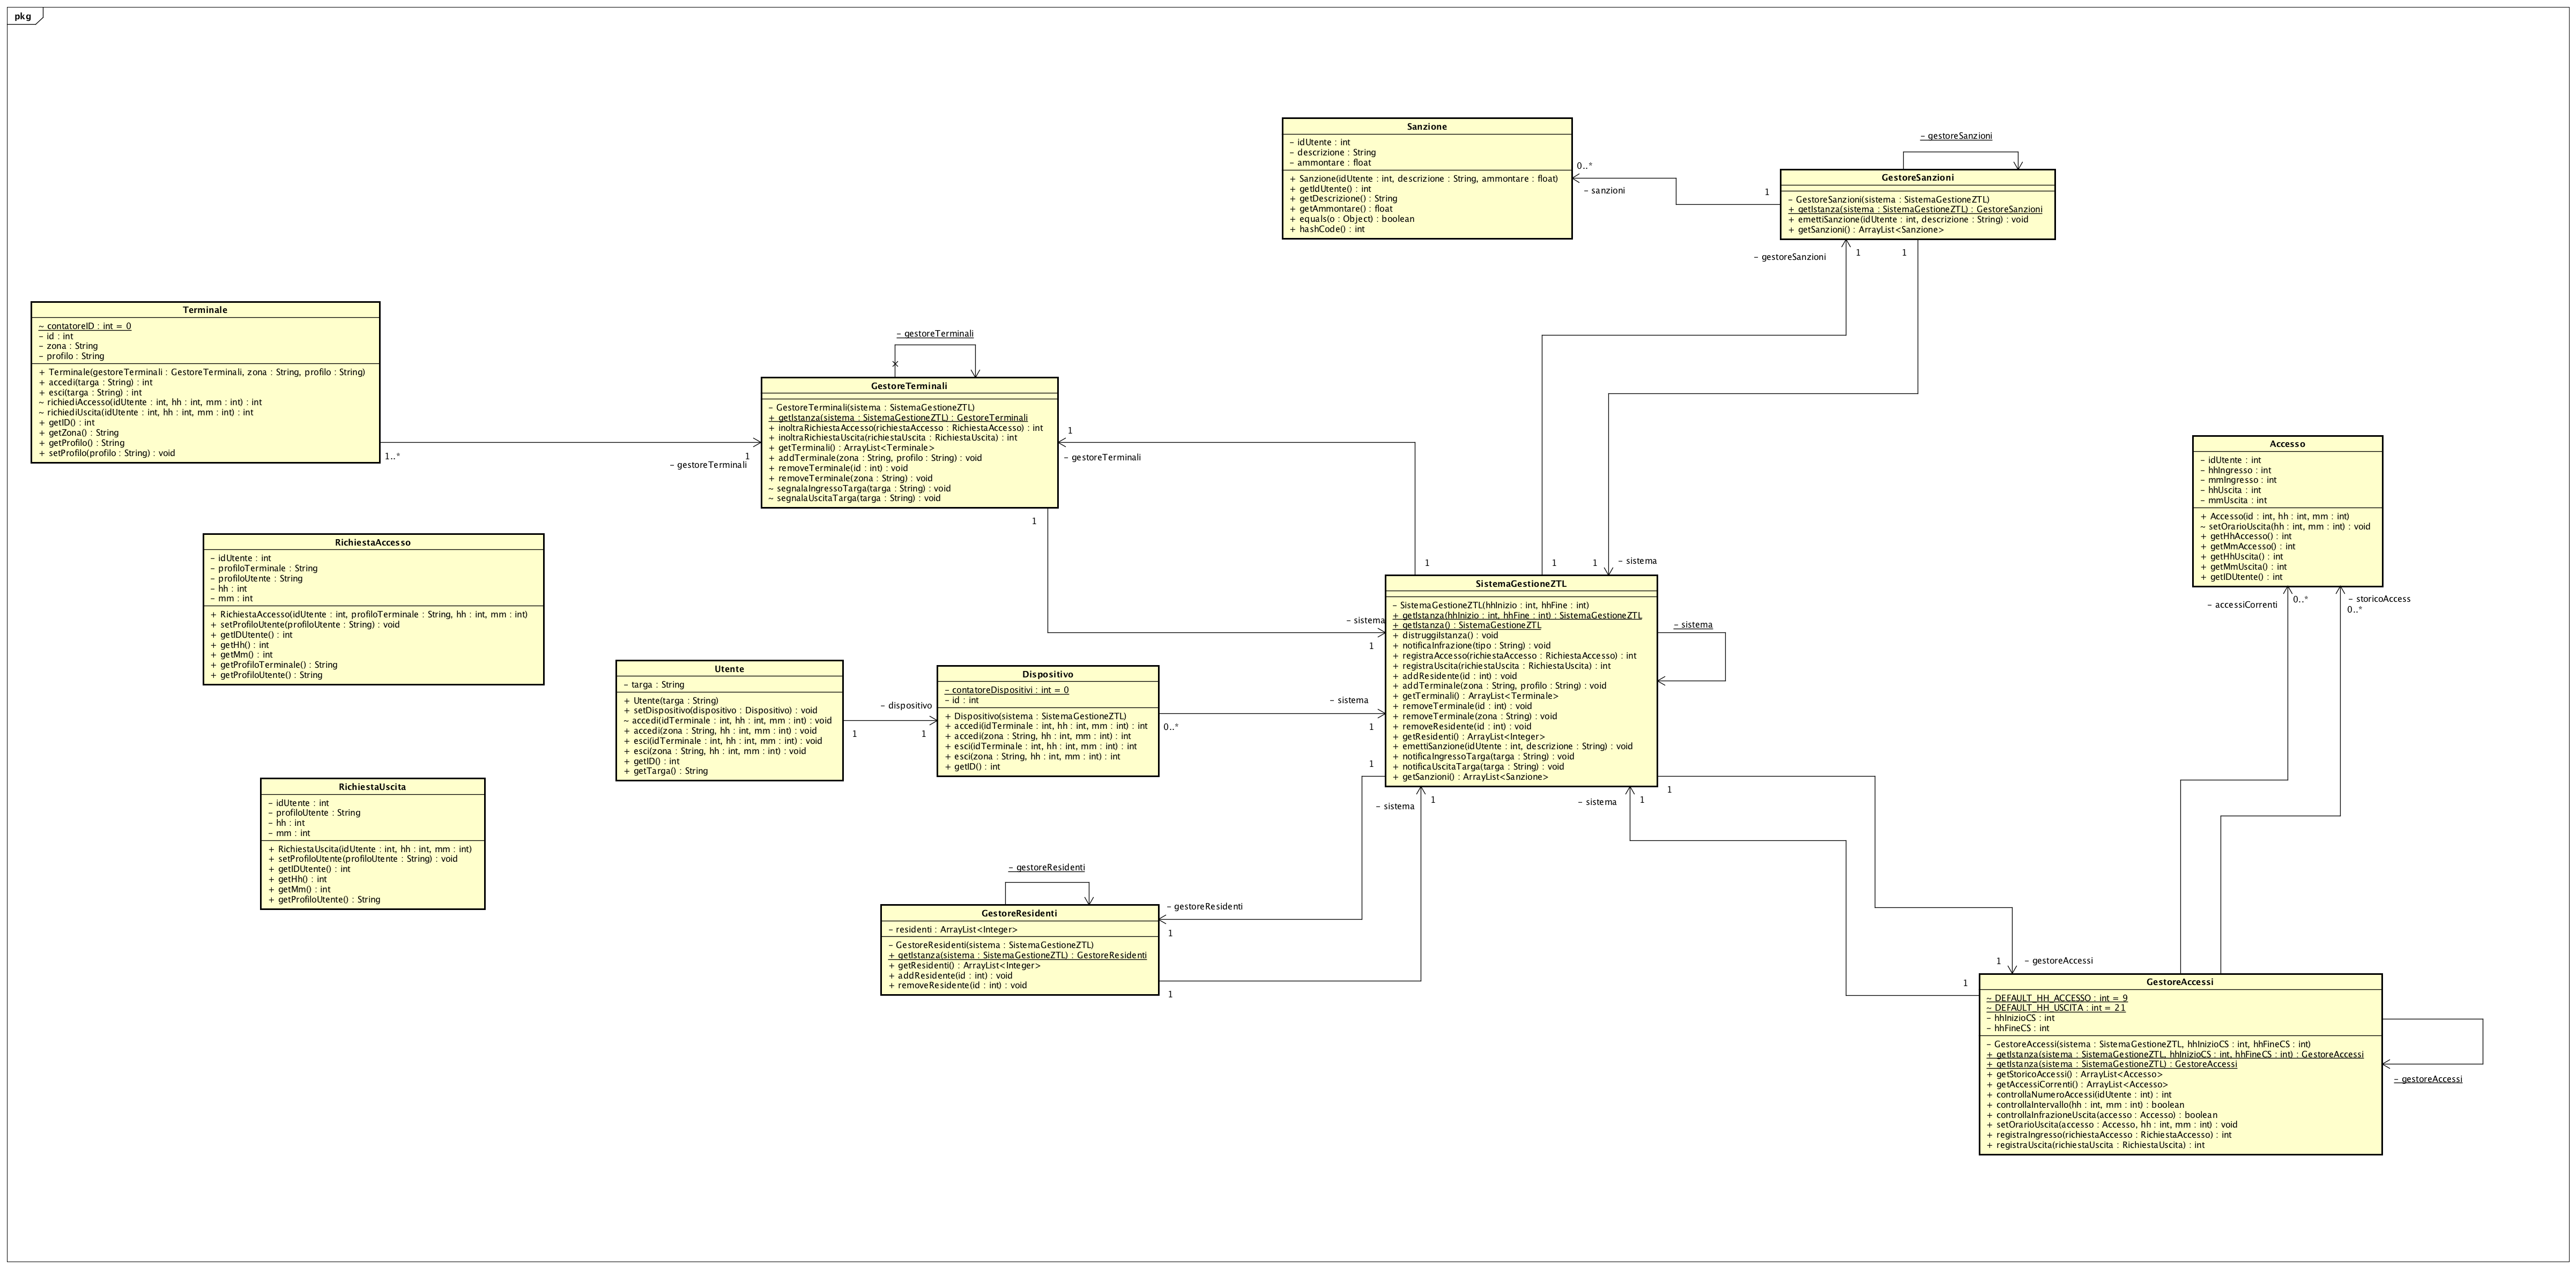
\includegraphics[scale=0.10]{DiagrammaClassi}
\end{figure} 

\noindent
Consultare i file \texttt{DiagrammaClassi.asta} e/o 
\texttt{DiagrammaClassi.png} per un maggiore dettaglio 
grafico

\section{Motivazioni progettuali}

\subsection{Riduzione dell'accoppiamento 
tramite \emph{Controller}}
Nonostante i sotto-componenti siano gestite dai
componenti gestori principali, notiamo che esse rimangono 
accoppiate al sistema centrale.
Pertanto le comunicazioni al sistema centrale passeranno
dai gestori in modo tale che le componenti rimangano 
accoppiate solamente ai gestori, e non al sistema centrale.

\subsection{Incapsulare richieste d'accesso/uscita}
La richiesta viene incapsulata in una classe 
per consentire di astrarre ulteriormente 
l'applicazione e per permettere un'agevole 
creazione delle relative istanze.

\subsection{Interfaccia Utente migliorata}
Sebbene l'interfaccia sia a riga di comando,
abbiamo aggiunto un'interfaccia funzionale, anch'essa 
componente che utilizzera il sistema centrale come mediatore 
per le sue richieste. Questo ci permetterà di avere un 
sistema, dove grazie anche all'aggiunta della classe 
\emph{Utente}, ci permetterà di simulare a pieno la zona 
a traffico limitato, ed il suo funzionamento a fronte 
delle varie interazioni. Le operazioni \emph{CRUD} 
saranno eseguite tramite essa.

\section{Casi di Test}
In questa iterazione, verificheremo
che le sanzioni ricevute siano quelle giuste 
e testeremo ancora che le funzioni che controllano 
gli intervalli siano corrette. In particolare,
queste ultime verranno testate con opportuni test 
unitari, mentre le altre con test di integrazione,
dato che coinvolgono diverse parti di sistema.

\noindent
A differenza delle altre iterazioni, vogliamo 
incrementare il numero di test in modo da 
garantire un più ampio test coverage, per quanto 
riguarda i test unitari e di integrazione.
La presenza di un ambiente di simulazione
permetterà di eseguire altre simulazioni per 
verificare che il sistema funzioni in maniera 
soddisfacente.

\subsection{Test Unitari della classe \emph{GestoreAccessi}}
Di questa classe, è di nostro interesse testare i metodi 
\texttt{controllaIntervallo()} e 
\texttt{controllaInfrazioneUscita()}. Ricordiamo che,
nei test, il sistema ammette utenti carico scarico dalle 
9 alle 21.
I casi di test scelti sono i seguenti:
\begin{itemize}
    \item L'orario 9:00 dovrà dare \texttt{true}
    \item L'orario 8:59 dovrà dare \texttt{false}
    \item L'orario 21:00 dovrà dare \texttt{true}
    \item L'orario 21:01 dovrà dare \texttt{false}
\end{itemize}

\noindent
Scegliamo, analogamente, dei casi di test che garantiscano
che il codice sia raggiunto in una buona percentuale:
\begin{itemize}
    \item L'intervallo 9:00 - 10:00 dovrà dare \texttt{true}
    \item L'intervallo 9:00 - 10:01 dovrà dare \texttt{false}
    \item L'intervallo 9:00 - 9:59 dovrà dare \texttt{true}
    \item L'intervallo 21:00 - 22:00 dovrà dare \texttt{true}
    \item L'intervallo 21:00 - 22:01 dovrà dare \texttt{false}
    \item L'intervallo 21:00 - 21:59 dovrà dare \texttt{true}
\end{itemize}

\subsection{Test d'integrazione di \emph{GestoreSanzioni}}
Per i seguenti test, vengono testate, per un utente ipotetico 
di ID 0, che le sanzioni emesse per lui in seguito a tutte 
le possibili cause, siano presenti nella lista.
Per fare ciò si istanziano le sanzioni dalla classe 
\emph{Sanzione} e viene controllata la lista per verificare 
che esistano le sanzioni istanziate, con i corretti valori.

\subsection{Test d'integrazione di \emph{Dispositivo}}
I casi che andremo a verificare per \texttt{accedi()} sono:
\begin{itemize}
    \item Utente CS entra da terminale CS alle 8:59, e darà -1
    \item Utente RES entra da terminale CS alle 8:59, e darà l'ID 
    \item Utente CS entra da terminale CS alle 9:00, e darà l'ID 
    \item Utente CS entra da terminale CS alle 21:00, e darà l'ID 
    \item Utente CS entra da terminale CS alle 21:01, e darà -1
    \item Utente RES entra da terminale RES alle 2:59, e darà l'ID 
    \item Utente CS entra da terminale RES alle 11:00, e darà -1
\end{itemize}

\noindent
Mentre i casi che verificheremo per \texttt{esci()} sono:
\begin{itemize}
    \item Utente CS (9:11 - 10:11), che darà l'ID 
    \item Utente CS (21:00 - 22:01), che darà -1
    \item Utente CS (21:00 - 22:00), che darà l'ID 
    \item Utente CS (11:00 - 17:00), che darà l'ID 
\end{itemize}

\end{document}